\documentclass[../main.tex]{subfile}
\begin{document}
\section{Simulations and results}
In the last chapters we introduced the theoretical background of superconductivity and altermagnets. 
The goal of this thesis is to use numerical methods to solve self-consitently the superconductive gap.
We remind here that all the code is available on a GitHub repository at \url{https://github.com/Tamwyn001/Thesis}.\\

\subsection{Methodology}
We're here going to simulate the s-wave superconductivity in a two-dimensional lattice,
in a superconductor and a junction of a superconductor and an altermagnet. 
The orientation of the interface can play some role in the behaviour of the superconducting gap, which 
makes the study of a straight and diagonal interface a case of study of particular interest. 
Further we will illustrate how the phase gradient of the gap can induce a current in the superconductor.
The shape of the d-wave gap parameter is also of interest. However, we missed the time to make a comprehensive study of it.
The de Josephon effect in an SC-AM-SC trilayer is in the code as well but need to be reworked.\\
\\    

The repository contains the Matlab code (.m) used to generate the data in the form of (coordinate, value) files (.dat).
Gnuplot scripts (.gp) allow us to produce some plots that we can then directly link to the Latex source code
of this thesis. Finally, some PowerShell scripts (.ps1) automate the gnuplot-latex process.\\

The Matlab code contains two important files. The system.m file is a class that describes which
 material we are using for the lattice, the physical context like the temperature and the chemical potential
as well as the use or not of periodic boundary conditions. It contains also the Hamiltonian of the system
and keeps track of all lattice sites.\\
The LaticeSites.m describes the position of a lattice sites, stores its neighbours and monitor the lattice
site specific physical quantities. These can be the superconducting gap or the current for instance.\\

We introduced earlier the need of a self-consistent solution for the gap to correctly describe the Hamiltonian.
This is achieved in the GapEquation.m file which is the main script we run. We start with a guess for
$\Delta_i$ and introduce it in the Hamiltonian. This guess can depend on the material, or the site 
if we aim to introduce some phase shift at specific locations.
We then derive a new site-dependent value using Eq. \ref{eq:SelfConsitentDelta} for all site and
reinsert it into the Hamiltonian. This requires to compute the eigenvectors and values of the Hamiltonian. This loop will be 
performed until the difference of each gap with its previous value reaches a threshold. We then have a proper 
Hamiltonian and can start to derivate some values like the current. \\

Matlab is a program that works well with matrices, so the choice was preferred during the prototyping. However, later in the process the fact that Matlab works 
by values and not by reference made quite some complications. Instead of passing a reference to location a variable is stored at,
we just copy it and pass it over. Here is an example: We have for each sites up to four neighbours. When computing the current divergence, 
we need the current of the neighbours. If we were to use reference method, then the lattice sites will be fixed defined in the memory,
and we can read it from all the places. However since we work by values, we need to send the values in each copy of the site.
So we have an array storing the lattice sites in the system, and another for each lattice point storing its neighbours.
However, these sites \textit{are the same entities}. Working by value means we need to set explicitly the value everywhere a site a stored.
Working by reference would have just need to set the value where the site is stored in the memory,
allowing all the references that points to this location being implicitly updated. In this sense a wiser choice would have been C++
with an appropriated diagonalization library. \\

The site coordinate is stored as $(x,y)$-tuple as well as an index $i$ that iterates over $y$-row and then starts again
at the beginning of the next row. This means that with different boundary conditions we get the following shape for the system:\\
\begin{figure}[H]
    \centering
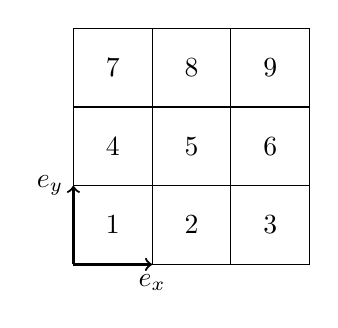
\begin{tikzpicture}
    \coordinate (o) at (0.5,0.5);
    \coordinate (x) at (1.5,0.5);
    \coordinate (y) at (0.5,1.5);

    \foreach \x in {1,2,3}
    {
        \foreach \y in {1,2,3}
        {
            \draw[fill=white] (\x-0.5,\y-0.5) rectangle (\x+0.5,\y+0.5);
            \node[anchor=center] at (\x,\y) {\pgfmathparse{int((\y-1)*3+\x)}\pgfmathresult};
        }
    } 
    \draw[->, thick] (o) -- (x) node[anchor = north]{$\bm{e}_x$};
    \draw[->, thick] (o) -- (y) node[anchor = east]{$\bm{e}_y$};
\end{tikzpicture}
\hspace{0.1\textwidth}
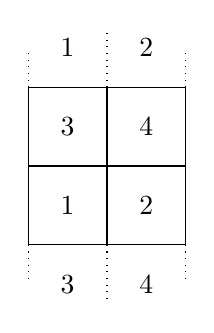
\begin{tikzpicture}
    \coordinate (topL) at (0.5,2.5);
    \coordinate (topM) at (1.5,2.5);
    \coordinate (topR) at (2.5,2.5);

    \foreach \x in {1,2}
    {
        \foreach \y in {1,2}
        {
            \draw[fill=white] (\x-0.5,\y-0.5) rectangle (\x+0.5,\y+0.5);

        }
    } 
    \draw[-, dotted] (topL) -- ++(0,0.5);
    \draw[-, dotted] (topM) -- ++(0,0.75);
    \draw[-, dotted] (topR) -- ++(0,0.5);

    \draw[-, dotted] (topL)++(0,-2) -- ++(0,-0.5);
    \draw[-, dotted] (topM)++(0,-2) -- ++(0,-0.75);
    \draw[-, dotted] (topR)++(0,-2) -- ++(0,-0.5);

    \node[anchor=center] at (1,1) {1};
    \node[anchor=center] at (2,1) {2};
    \node[anchor=center] at (1,2) {3};
    \node[anchor=center] at (2,2) {4};
    \node[anchor=center] at (1,3) {1};
    \node[anchor=center] at (2,3) {2};
    \node[anchor=center] at (1,0) {3};
    \node[anchor=center] at (2,0) {4};


\end{tikzpicture}
\hspace{0.1\textwidth}
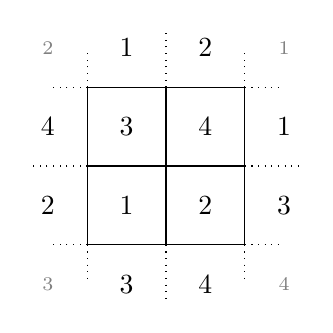
\begin{tikzpicture}
    \coordinate (topL) at (0.5,2.5);
    \coordinate (topM) at (1.5,2.5);
    \coordinate (topR) at (2.5,2.5);

    \coordinate (sideL) at (0.5,0.5);
    \coordinate (sideM) at (0.5,1.5);
    \coordinate (sideR) at (0.5,2.5);

    \foreach \x in {1,2}
    {
        \foreach \y in {1,2}
        {
            \draw[fill=white] (\x-0.5,\y-0.5) rectangle (\x+0.5,\y+0.5);

        }
    } 
    \draw[-, dotted] (topL) -- ++(0,0.5);
    \draw[-, dotted] (topM) -- ++(0,0.75);
    \draw[-, dotted] (topR) -- ++(0,0.5);

    \draw[-, dotted] (topL)++(0,-2) -- ++(0,-0.5);
    \draw[-, dotted] (topM)++(0,-2) -- ++(0,-0.75);
    \draw[-, dotted] (topR)++(0,-2) -- ++(0,-0.5);

    \draw[-, dotted] (sideL) -- ++(-0.5,0);
    \draw[-, dotted] (sideM) -- ++(-0.75,0);
    \draw[-, dotted] (sideR) -- ++(-0.5,0);

    \draw[-, dotted] (sideL)++(2,0) -- ++(0.5,0);
    \draw[-, dotted] (sideM)++(2,0) -- ++(0.75,0);
    \draw[-, dotted] (sideR)++(2,0) -- ++(0.5,0);

    \node[anchor=center] at (1,1) {1};
    \node[anchor=center] at (2,1) {2};
    \node[anchor=center] at (1,2) {3};
    \node[anchor=center] at (2,2) {4};

    \node[anchor=center] at (1,3) {1};
    \node[anchor=center] at (2,3) {2};
    \node[anchor=center] at (1,0) {3};
    \node[anchor=center] at (2,0) {4};

    \node[anchor=center] at (3,2) {1};
    \node[anchor=center] at (3,1) {3};
    \node[anchor=center] at (0,1) {2};
    \node[anchor=center] at (0,2) {4};

    \node[anchor=center, color = gray] at (3,3) {\scriptsize 1};
    \node[anchor=center, color = gray] at (0,3) {\scriptsize 2};
    \node[anchor=center, color = gray] at (0,0) {\scriptsize 3};
    \node[anchor=center, color = gray] at (3,0) {\scriptsize 4};

\end{tikzpicture}
\caption{The sites indexing method as well as a representation of the different boundary conditions.}
\label{fig:Sim_System}
\end{figure}
Left we have a $3\times3$-system. The others are $2\times2$ with vertical periodic boundary conditions (PBC)
and on the right with both vertical and horizontal PBC.\\

\paragraph{Mathematical definition of PBCs}$~$\\

We have a rectangular lattice of size $N_x\times N_y$. The quantities have to be the same on both side of the system along the axis having these PBC.
Here we have vertical periodic boundary conditions. This means that the quantities have to be the same on the top and the bottom of the system. 
If we describe the system with a wavefunction $\Psi(x,y)$ then we have:
\begin{equation}
    \Psi(x,y) = \Psi(x,y+N_y) \quad\quad \forall x\in\natset{N_x}\quad, \forall y \in \natset{N_y}
\end{equation} 
This leads to a finite number of possibility for the Fourier transform of the wavefunction, as we are going to show in Sec. \ref{sec:Vertical_Fourier}.\\

We want to maximize the definition of the gap in the lattice. With the architecture we have (Intel i7 11th gen, 8 GB RAM),
an upper bound of $40\times20=1200$ sites was achieved. Matlab being an interpreter, this could be optimized by using a compiled language.
In the literature we find square lattices of $100\times100$ sites being used \cite{Mjos2019}. We compute with a convergence threshold of \num{1.0e-3}. \\
% \subsection{Results}
% \subsection{Gap parameter}
% As we saw, the gap parameter is the key value to solve before considering computing anything else.
% Following the description of \ref{eq:SelfConsitentDelta}, we see that because of $U_i$, this value should only exist 
% in the superconductor. We thefore start by taking a long superconductor (SC) having 30 lattice site in $\bm{e}_x$ and $\bm{e}_y$. 
% However later studies are going to show that the the expectation value $\langle c_{i\uparrow} c_{i\downarrow}\rangle$ is not
% only defined in the SC. This expectation value can be seen as a Cooper-pair density. \rem{true statment?}.
% Later we are going to stack some layer on the $\bm{e}_x$ axis, so we first achieve a plot showing the gap on each $\bm{e}_x$-slice
% by averaging on the $\bm{e}_y$ axis to a given $\bm{e}_x$. To stay consitent, we are therfore going to plot only the expectation
% part of the gap $\Delta$. However $U_i$ is setted to be one in an SC, so it doesn't make a big difference in a SC.

% \begin{figure}[H]
%     \centering
%     % GNUPLOT: LaTeX picture with Postscript
\begingroup
  % Encoding inside the plot.  In the header of your document, this encoding
  % should to defined, e.g., by using
  % \usepackage[cp1252,<other encodings>]{inputenc}
  \inputencoding{cp1252}%
  \makeatletter
  \providecommand\color[2][]{%
    \GenericError{(gnuplot) \space\space\space\@spaces}{%
      Package color not loaded in conjunction with
      terminal option `colourtext'%
    }{See the gnuplot documentation for explanation.%
    }{Either use 'blacktext' in gnuplot or load the package
      color.sty in LaTeX.}%
    \renewcommand\color[2][]{}%
  }%
  \providecommand\includegraphics[2][]{%
    \GenericError{(gnuplot) \space\space\space\@spaces}{%
      Package graphicx or graphics not loaded%
    }{See the gnuplot documentation for explanation.%
    }{The gnuplot epslatex terminal needs graphicx.sty or graphics.sty.}%
    \renewcommand\includegraphics[2][]{}%
  }%
  \providecommand\rotatebox[2]{#2}%
  \@ifundefined{ifGPcolor}{%
    \newif\ifGPcolor
    \GPcolortrue
  }{}%
  \@ifundefined{ifGPblacktext}{%
    \newif\ifGPblacktext
    \GPblacktextfalse
  }{}%
  % define a \g@addto@macro without @ in the name:
  \let\gplgaddtomacro\g@addto@macro
  % define empty templates for all commands taking text:
  \gdef\gplbacktext{}%
  \gdef\gplfronttext{}%
  \makeatother
  \ifGPblacktext
    % no textcolor at all
    \def\colorrgb#1{}%
    \def\colorgray#1{}%
  \else
    % gray or color?
    \ifGPcolor
      \def\colorrgb#1{\color[rgb]{#1}}%
      \def\colorgray#1{\color[gray]{#1}}%
      \expandafter\def\csname LTw\endcsname{\color{white}}%
      \expandafter\def\csname LTb\endcsname{\color{black}}%
      \expandafter\def\csname LTa\endcsname{\color{black}}%
      \expandafter\def\csname LT0\endcsname{\color[rgb]{1,0,0}}%
      \expandafter\def\csname LT1\endcsname{\color[rgb]{0,1,0}}%
      \expandafter\def\csname LT2\endcsname{\color[rgb]{0,0,1}}%
      \expandafter\def\csname LT3\endcsname{\color[rgb]{1,0,1}}%
      \expandafter\def\csname LT4\endcsname{\color[rgb]{0,1,1}}%
      \expandafter\def\csname LT5\endcsname{\color[rgb]{1,1,0}}%
      \expandafter\def\csname LT6\endcsname{\color[rgb]{0,0,0}}%
      \expandafter\def\csname LT7\endcsname{\color[rgb]{1,0.3,0}}%
      \expandafter\def\csname LT8\endcsname{\color[rgb]{0.5,0.5,0.5}}%
    \else
      % gray
      \def\colorrgb#1{\color{black}}%
      \def\colorgray#1{\color[gray]{#1}}%
      \expandafter\def\csname LTw\endcsname{\color{white}}%
      \expandafter\def\csname LTb\endcsname{\color{black}}%
      \expandafter\def\csname LTa\endcsname{\color{black}}%
      \expandafter\def\csname LT0\endcsname{\color{black}}%
      \expandafter\def\csname LT1\endcsname{\color{black}}%
      \expandafter\def\csname LT2\endcsname{\color{black}}%
      \expandafter\def\csname LT3\endcsname{\color{black}}%
      \expandafter\def\csname LT4\endcsname{\color{black}}%
      \expandafter\def\csname LT5\endcsname{\color{black}}%
      \expandafter\def\csname LT6\endcsname{\color{black}}%
      \expandafter\def\csname LT7\endcsname{\color{black}}%
      \expandafter\def\csname LT8\endcsname{\color{black}}%
    \fi
  \fi
    \setlength{\unitlength}{0.0500bp}%
    \ifx\gptboxheight\undefined%
      \newlength{\gptboxheight}%
      \newlength{\gptboxwidth}%
      \newsavebox{\gptboxtext}%
    \fi%
    \setlength{\fboxrule}{0.5pt}%
    \setlength{\fboxsep}{1pt}%
    \definecolor{tbcol}{rgb}{1,1,1}%
\begin{picture}(5760.00,3772.00)%
    \gplgaddtomacro\gplbacktext{%
      \csname LTb\endcsname%%
      \put(1807,3313){\makebox(0,0){\strut{}SC}}%
      \put(3953,3313){\makebox(0,0){\strut{}AM}}%
    }%
    \gplgaddtomacro\gplfronttext{%
      \csname LTb\endcsname%%
      \put(1073,742){\makebox(0,0){\scriptsize 2}}%
      \put(1525,742){\makebox(0,0){\scriptsize 4}}%
      \put(1977,742){\makebox(0,0){\scriptsize 6}}%
      \put(2429,742){\makebox(0,0){\scriptsize 8}}%
      \put(2880,742){\makebox(0,0){\scriptsize 10}}%
      \put(3331,742){\makebox(0,0){\scriptsize 12}}%
      \put(3783,742){\makebox(0,0){\scriptsize 14}}%
      \put(4235,742){\makebox(0,0){\scriptsize 16}}%
      \put(4687,742){\makebox(0,0){\scriptsize 18}}%
      \put(2880,478){\makebox(0,0){\small\textbf{Lattice site $i_x$ in $\bm{e}_x$}}}%
      \put(480,1006){\makebox(0,0){\scriptsize 2}}%
      \put(480,1254){\makebox(0,0){\scriptsize 4}}%
      \put(480,1501){\makebox(0,0){\scriptsize 6}}%
      \put(480,1749){\makebox(0,0){\scriptsize 8}}%
      \put(480,1996){\makebox(0,0){\scriptsize 10}}%
      \put(480,2243){\makebox(0,0){\scriptsize 12}}%
      \put(480,2491){\makebox(0,0){\scriptsize 14}}%
      \put(480,2738){\makebox(0,0){\scriptsize 16}}%
      \put(480,2986){\makebox(0,0){\scriptsize 18}}%
      \put(150,1996){\rotatebox{-270.00}{\makebox(0,0){\small\textbf{Lattice site $i_y$ in $\bm{e}_y$}}}}%
      \put(5743,820){\makebox(0,0){\tiny \(0\)}}%
      \put(5743,1212){\makebox(0,0){\tiny \(1e{-06}\)}}%
      \put(5743,1604){\makebox(0,0){\tiny \(2e{-06}\)}}%
      \put(5743,1996){\makebox(0,0){\tiny \(3e{-06}\)}}%
      \put(5743,2388){\makebox(0,0){\tiny \(4e{-06}\)}}%
      \put(5743,2780){\makebox(0,0){\tiny \(5e{-06}\)}}%
      \put(5743,3171){\makebox(0,0){\tiny \(6e{-06}\)}}%
    }%
    \gplbacktext
    \put(0,0){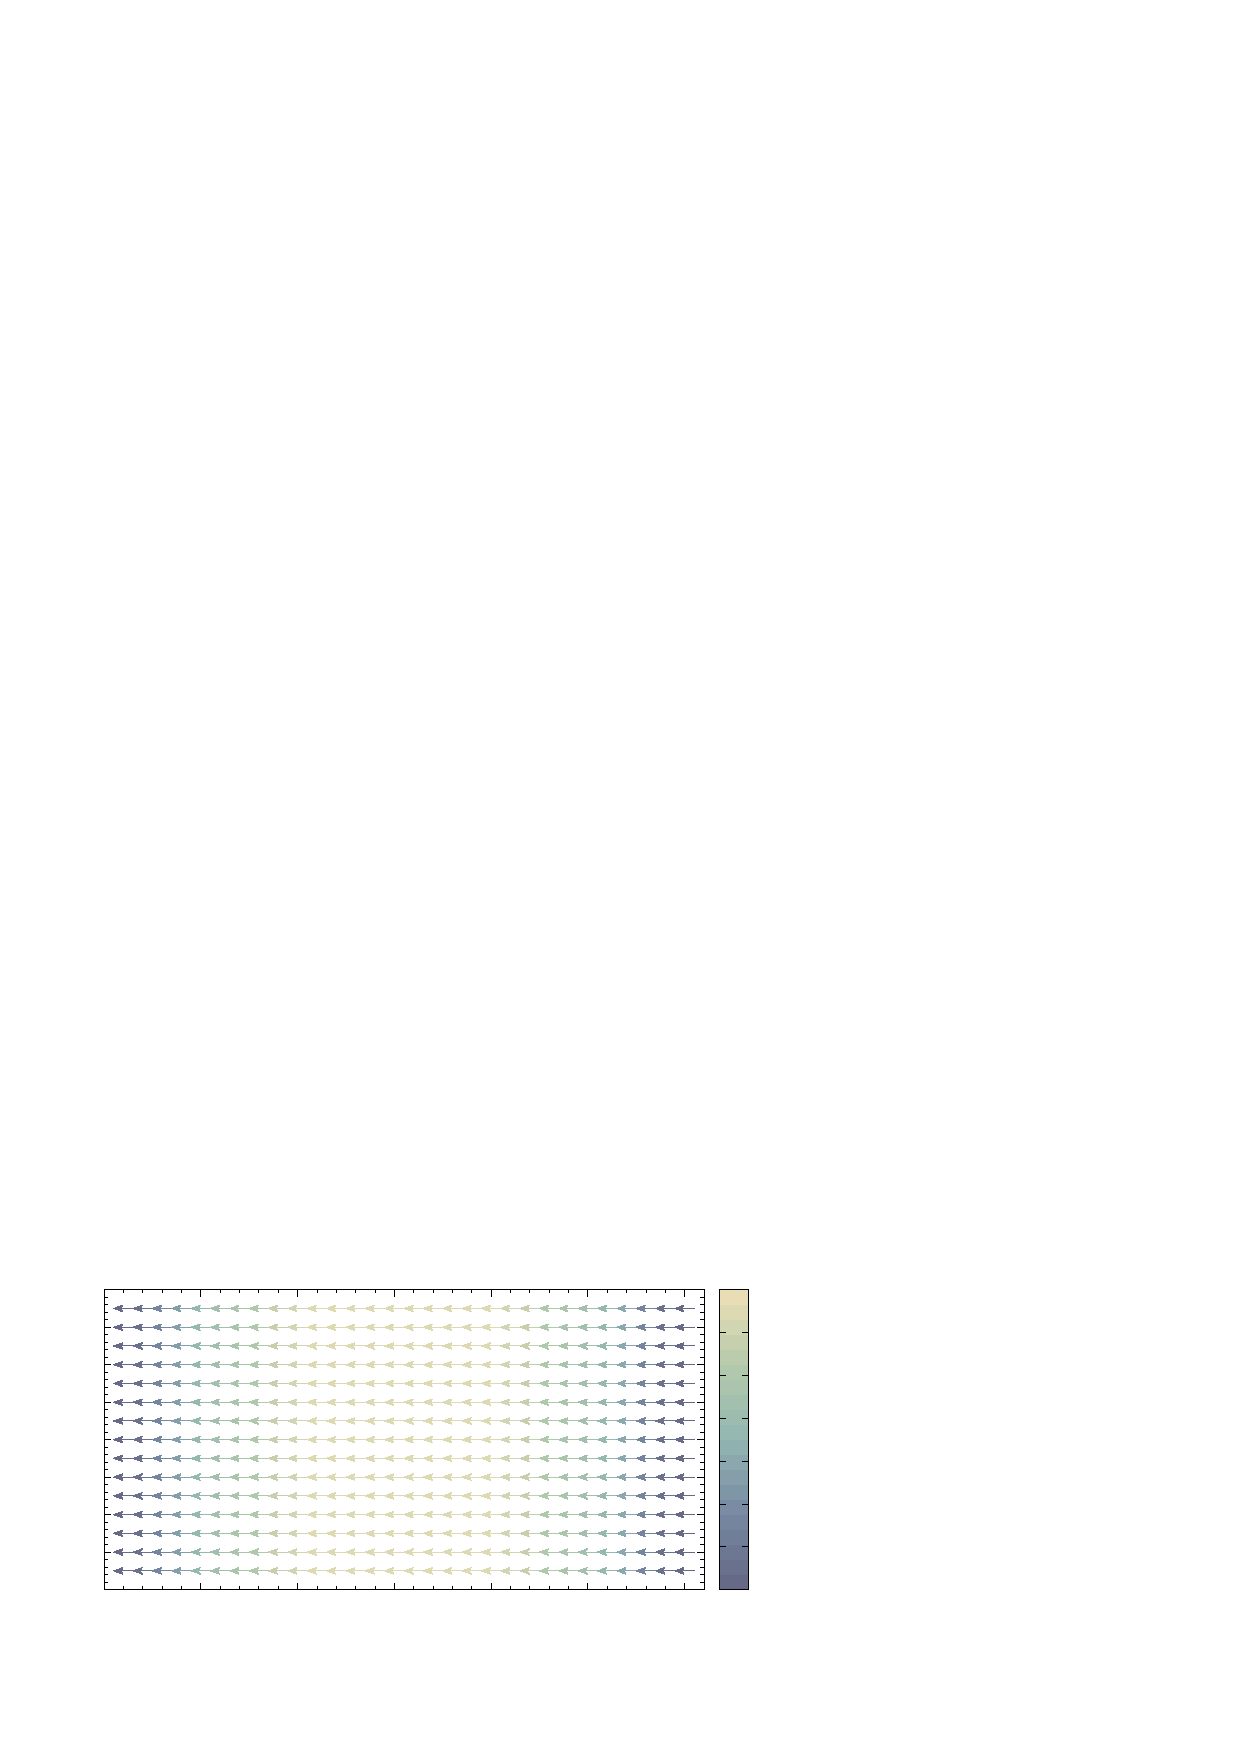
\includegraphics[width={288.00bp},height={188.60bp}]{Plots/SC10AM10/HeatMap/VertHorizBC/plot}}%
    \gplfronttext
  \end{picture}%
\endgroup


%     \caption{Mean value over the $y$-axis of the correlation function $|\langle c_{i\uparrow} c_{i\downarrow}\rangle|$ for different
%      boundary conditions in a SC. \rem{remove the logscale}}
% \end{figure} 
% The gap is almost the same for the different boundary conditions (BC). When having vaccum on the left and right side of the 
% material we observe a drop in the gap. This is due to the fect that on these sites the interaction occures with at most three
% neighbours (two for the corners when no BC). Whereas there are four neighbours on the other locations, inside the material.
% In contrast, for an inflinitly-long superconductor in the $\bm{e}_x$
% direction, $\Delta$ approaches a constant value. In this context every site interacts with four others. \\

% The next step would be to snap an altermagnets next to the superconductor an plot the same quantity.
% \begin{figure}[H]
%     \centering
%     % GNUPLOT: LaTeX picture with Postscript
\begingroup
  % Encoding inside the plot.  In the header of your document, this encoding
  % should to defined, e.g., by using
  % \usepackage[cp1252,<other encodings>]{inputenc}
  \inputencoding{cp1252}%
  \makeatletter
  \providecommand\color[2][]{%
    \GenericError{(gnuplot) \space\space\space\@spaces}{%
      Package color not loaded in conjunction with
      terminal option `colourtext'%
    }{See the gnuplot documentation for explanation.%
    }{Either use 'blacktext' in gnuplot or load the package
      color.sty in LaTeX.}%
    \renewcommand\color[2][]{}%
  }%
  \providecommand\includegraphics[2][]{%
    \GenericError{(gnuplot) \space\space\space\@spaces}{%
      Package graphicx or graphics not loaded%
    }{See the gnuplot documentation for explanation.%
    }{The gnuplot epslatex terminal needs graphicx.sty or graphics.sty.}%
    \renewcommand\includegraphics[2][]{}%
  }%
  \providecommand\rotatebox[2]{#2}%
  \@ifundefined{ifGPcolor}{%
    \newif\ifGPcolor
    \GPcolortrue
  }{}%
  \@ifundefined{ifGPblacktext}{%
    \newif\ifGPblacktext
    \GPblacktextfalse
  }{}%
  % define a \g@addto@macro without @ in the name:
  \let\gplgaddtomacro\g@addto@macro
  % define empty templates for all commands taking text:
  \gdef\gplbacktext{}%
  \gdef\gplfronttext{}%
  \makeatother
  \ifGPblacktext
    % no textcolor at all
    \def\colorrgb#1{}%
    \def\colorgray#1{}%
  \else
    % gray or color?
    \ifGPcolor
      \def\colorrgb#1{\color[rgb]{#1}}%
      \def\colorgray#1{\color[gray]{#1}}%
      \expandafter\def\csname LTw\endcsname{\color{white}}%
      \expandafter\def\csname LTb\endcsname{\color{black}}%
      \expandafter\def\csname LTa\endcsname{\color{black}}%
      \expandafter\def\csname LT0\endcsname{\color[rgb]{1,0,0}}%
      \expandafter\def\csname LT1\endcsname{\color[rgb]{0,1,0}}%
      \expandafter\def\csname LT2\endcsname{\color[rgb]{0,0,1}}%
      \expandafter\def\csname LT3\endcsname{\color[rgb]{1,0,1}}%
      \expandafter\def\csname LT4\endcsname{\color[rgb]{0,1,1}}%
      \expandafter\def\csname LT5\endcsname{\color[rgb]{1,1,0}}%
      \expandafter\def\csname LT6\endcsname{\color[rgb]{0,0,0}}%
      \expandafter\def\csname LT7\endcsname{\color[rgb]{1,0.3,0}}%
      \expandafter\def\csname LT8\endcsname{\color[rgb]{0.5,0.5,0.5}}%
    \else
      % gray
      \def\colorrgb#1{\color{black}}%
      \def\colorgray#1{\color[gray]{#1}}%
      \expandafter\def\csname LTw\endcsname{\color{white}}%
      \expandafter\def\csname LTb\endcsname{\color{black}}%
      \expandafter\def\csname LTa\endcsname{\color{black}}%
      \expandafter\def\csname LT0\endcsname{\color{black}}%
      \expandafter\def\csname LT1\endcsname{\color{black}}%
      \expandafter\def\csname LT2\endcsname{\color{black}}%
      \expandafter\def\csname LT3\endcsname{\color{black}}%
      \expandafter\def\csname LT4\endcsname{\color{black}}%
      \expandafter\def\csname LT5\endcsname{\color{black}}%
      \expandafter\def\csname LT6\endcsname{\color{black}}%
      \expandafter\def\csname LT7\endcsname{\color{black}}%
      \expandafter\def\csname LT8\endcsname{\color{black}}%
    \fi
  \fi
    \setlength{\unitlength}{0.0500bp}%
    \ifx\gptboxheight\undefined%
      \newlength{\gptboxheight}%
      \newlength{\gptboxwidth}%
      \newsavebox{\gptboxtext}%
    \fi%
    \setlength{\fboxrule}{0.5pt}%
    \setlength{\fboxsep}{1pt}%
    \definecolor{tbcol}{rgb}{1,1,1}%
\begin{picture}(5760.00,3772.00)%
    \gplgaddtomacro\gplbacktext{%
      \csname LTb\endcsname%%
      \put(1807,3313){\makebox(0,0){\strut{}SC}}%
      \put(3953,3313){\makebox(0,0){\strut{}AM}}%
    }%
    \gplgaddtomacro\gplfronttext{%
      \csname LTb\endcsname%%
      \put(1073,742){\makebox(0,0){\scriptsize 2}}%
      \put(1525,742){\makebox(0,0){\scriptsize 4}}%
      \put(1977,742){\makebox(0,0){\scriptsize 6}}%
      \put(2429,742){\makebox(0,0){\scriptsize 8}}%
      \put(2880,742){\makebox(0,0){\scriptsize 10}}%
      \put(3331,742){\makebox(0,0){\scriptsize 12}}%
      \put(3783,742){\makebox(0,0){\scriptsize 14}}%
      \put(4235,742){\makebox(0,0){\scriptsize 16}}%
      \put(4687,742){\makebox(0,0){\scriptsize 18}}%
      \put(2880,478){\makebox(0,0){\small\textbf{Lattice site $i_x$ in $\bm{e}_x$}}}%
      \put(480,1006){\makebox(0,0){\scriptsize 2}}%
      \put(480,1254){\makebox(0,0){\scriptsize 4}}%
      \put(480,1501){\makebox(0,0){\scriptsize 6}}%
      \put(480,1749){\makebox(0,0){\scriptsize 8}}%
      \put(480,1996){\makebox(0,0){\scriptsize 10}}%
      \put(480,2243){\makebox(0,0){\scriptsize 12}}%
      \put(480,2491){\makebox(0,0){\scriptsize 14}}%
      \put(480,2738){\makebox(0,0){\scriptsize 16}}%
      \put(480,2986){\makebox(0,0){\scriptsize 18}}%
      \put(150,1996){\rotatebox{-270.00}{\makebox(0,0){\small\textbf{Lattice site $i_y$ in $\bm{e}_y$}}}}%
      \put(5743,820){\makebox(0,0){\tiny \(0\)}}%
      \put(5743,1212){\makebox(0,0){\tiny \(1e{-06}\)}}%
      \put(5743,1604){\makebox(0,0){\tiny \(2e{-06}\)}}%
      \put(5743,1996){\makebox(0,0){\tiny \(3e{-06}\)}}%
      \put(5743,2388){\makebox(0,0){\tiny \(4e{-06}\)}}%
      \put(5743,2780){\makebox(0,0){\tiny \(5e{-06}\)}}%
      \put(5743,3171){\makebox(0,0){\tiny \(6e{-06}\)}}%
    }%
    \gplbacktext
    \put(0,0){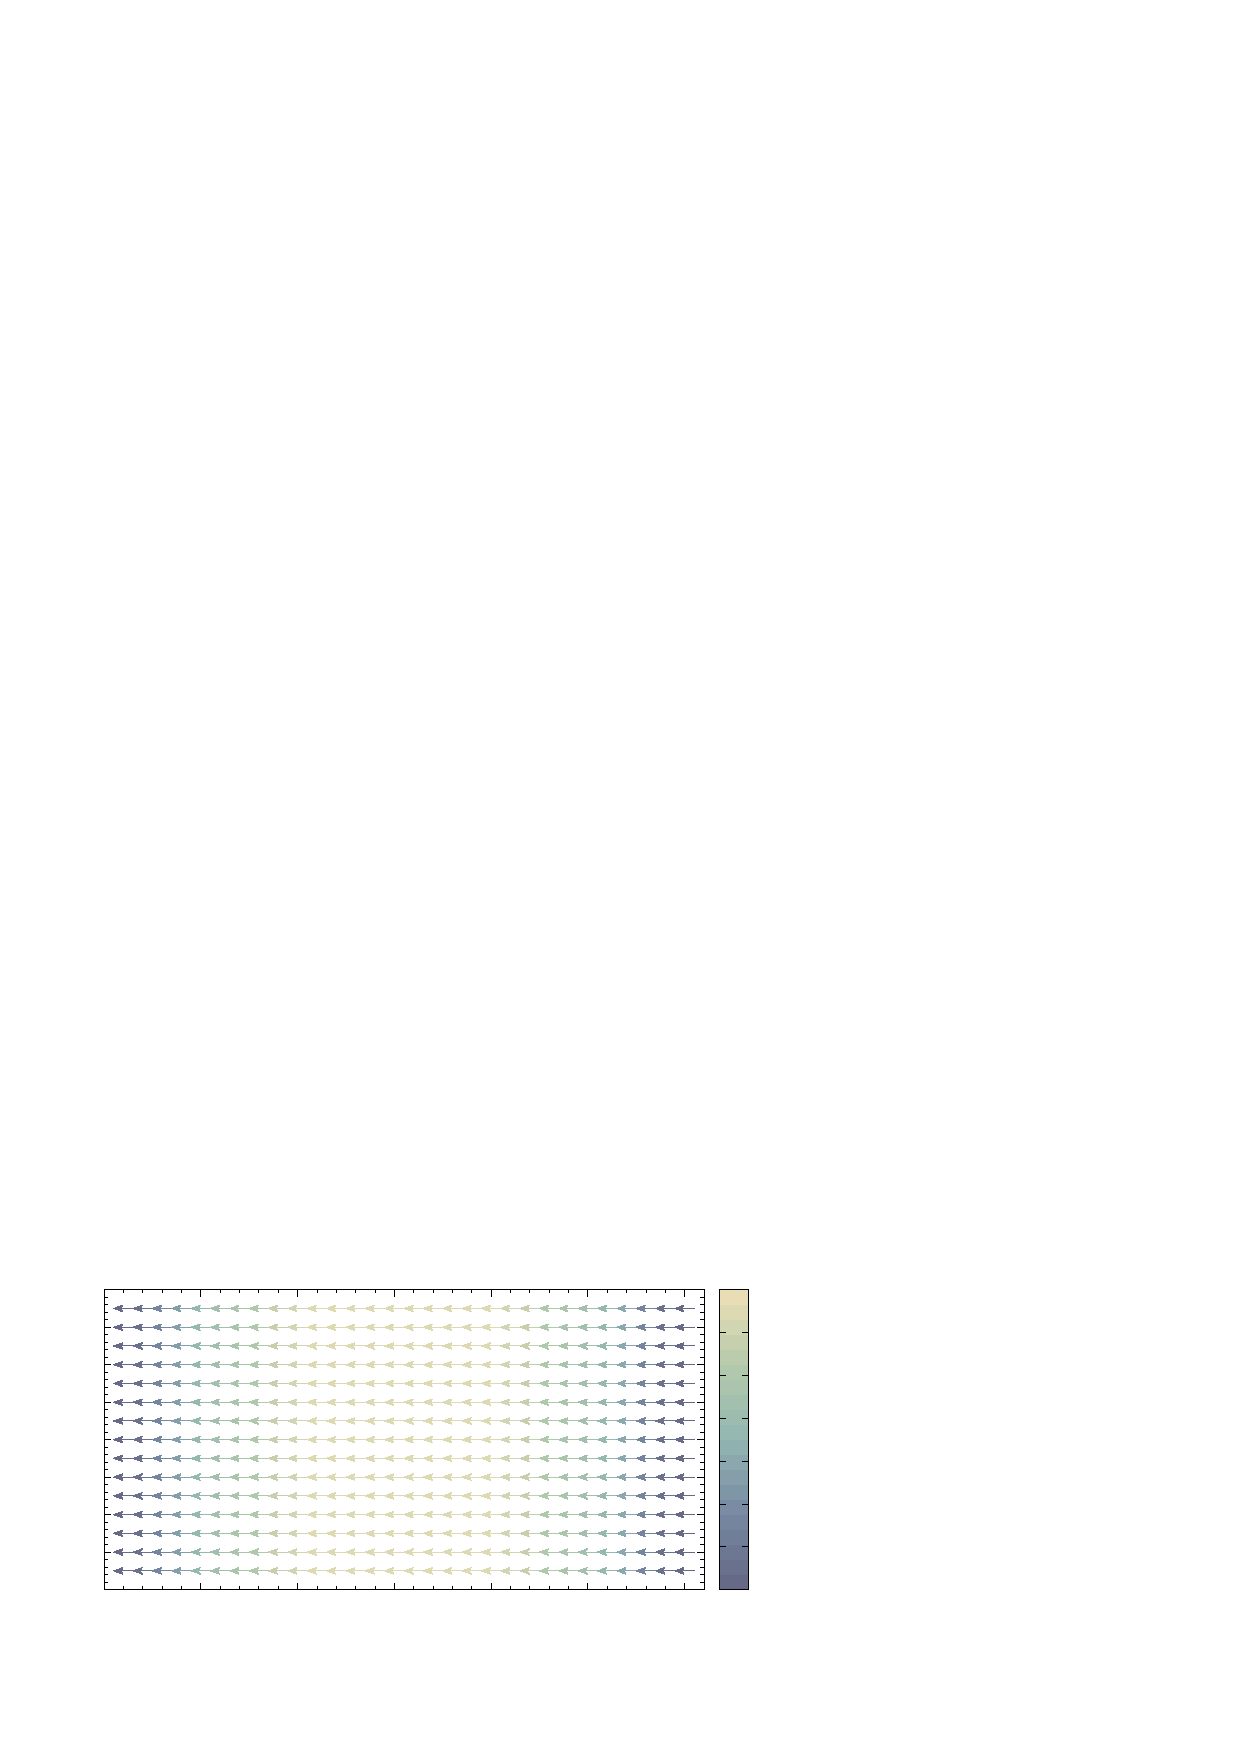
\includegraphics[width={288.00bp},height={188.60bp}]{Plots/SC10AM10/HeatMap/VertHorizBC/plot}}%
    \gplfronttext
  \end{picture}%
\endgroup


%     \caption{Mean value over the $y$-axis of the correlation function $|\langle c_{i\uparrow} c_{i\downarrow}\rangle|$ for different
%      boundary conditions in a SC and an AM.}
% \end{figure} 
% Taking into account the logarithmic scale on $|\langle c_{i\uparrow} c_{i\downarrow}\rangle|$, we see that without horizontal
% PBC the Cooper pairs leak into the altermagnet. Their density degrows expentialy with the ditance from the interface. Following
% this idea, whene enabling the horizontal PBC we allow two SC on both side of an AM. This results in this well form were we observe
% a leaking for the left and the right inside the AM. Some oscilations are also visible on the side of the SC for the vertical and 
% horizontal PBC case. These are known as [..] and results from [..] \rem{ask Jacob}.\\

% The repartition of the gap in real space is also intersting to look at. In fact the above averaging blends out the shape 
% of this value in the lattice.

% \begin{figure}[H]
%     \centering
%     \begin{subfigure}{0.3\textwidth}
%         \centering
%         % GNUPLOT: LaTeX picture with Postscript
\begingroup
  % Encoding inside the plot.  In the header of your document, this encoding
  % should to defined, e.g., by using
  % \usepackage[cp1252,<other encodings>]{inputenc}
  \inputencoding{cp1252}%
  \makeatletter
  \providecommand\color[2][]{%
    \GenericError{(gnuplot) \space\space\space\@spaces}{%
      Package color not loaded in conjunction with
      terminal option `colourtext'%
    }{See the gnuplot documentation for explanation.%
    }{Either use 'blacktext' in gnuplot or load the package
      color.sty in LaTeX.}%
    \renewcommand\color[2][]{}%
  }%
  \providecommand\includegraphics[2][]{%
    \GenericError{(gnuplot) \space\space\space\@spaces}{%
      Package graphicx or graphics not loaded%
    }{See the gnuplot documentation for explanation.%
    }{The gnuplot epslatex terminal needs graphicx.sty or graphics.sty.}%
    \renewcommand\includegraphics[2][]{}%
  }%
  \providecommand\rotatebox[2]{#2}%
  \@ifundefined{ifGPcolor}{%
    \newif\ifGPcolor
    \GPcolortrue
  }{}%
  \@ifundefined{ifGPblacktext}{%
    \newif\ifGPblacktext
    \GPblacktextfalse
  }{}%
  % define a \g@addto@macro without @ in the name:
  \let\gplgaddtomacro\g@addto@macro
  % define empty templates for all commands taking text:
  \gdef\gplbacktext{}%
  \gdef\gplfronttext{}%
  \makeatother
  \ifGPblacktext
    % no textcolor at all
    \def\colorrgb#1{}%
    \def\colorgray#1{}%
  \else
    % gray or color?
    \ifGPcolor
      \def\colorrgb#1{\color[rgb]{#1}}%
      \def\colorgray#1{\color[gray]{#1}}%
      \expandafter\def\csname LTw\endcsname{\color{white}}%
      \expandafter\def\csname LTb\endcsname{\color{black}}%
      \expandafter\def\csname LTa\endcsname{\color{black}}%
      \expandafter\def\csname LT0\endcsname{\color[rgb]{1,0,0}}%
      \expandafter\def\csname LT1\endcsname{\color[rgb]{0,1,0}}%
      \expandafter\def\csname LT2\endcsname{\color[rgb]{0,0,1}}%
      \expandafter\def\csname LT3\endcsname{\color[rgb]{1,0,1}}%
      \expandafter\def\csname LT4\endcsname{\color[rgb]{0,1,1}}%
      \expandafter\def\csname LT5\endcsname{\color[rgb]{1,1,0}}%
      \expandafter\def\csname LT6\endcsname{\color[rgb]{0,0,0}}%
      \expandafter\def\csname LT7\endcsname{\color[rgb]{1,0.3,0}}%
      \expandafter\def\csname LT8\endcsname{\color[rgb]{0.5,0.5,0.5}}%
    \else
      % gray
      \def\colorrgb#1{\color{black}}%
      \def\colorgray#1{\color[gray]{#1}}%
      \expandafter\def\csname LTw\endcsname{\color{white}}%
      \expandafter\def\csname LTb\endcsname{\color{black}}%
      \expandafter\def\csname LTa\endcsname{\color{black}}%
      \expandafter\def\csname LT0\endcsname{\color{black}}%
      \expandafter\def\csname LT1\endcsname{\color{black}}%
      \expandafter\def\csname LT2\endcsname{\color{black}}%
      \expandafter\def\csname LT3\endcsname{\color{black}}%
      \expandafter\def\csname LT4\endcsname{\color{black}}%
      \expandafter\def\csname LT5\endcsname{\color{black}}%
      \expandafter\def\csname LT6\endcsname{\color{black}}%
      \expandafter\def\csname LT7\endcsname{\color{black}}%
      \expandafter\def\csname LT8\endcsname{\color{black}}%
    \fi
  \fi
    \setlength{\unitlength}{0.0500bp}%
    \ifx\gptboxheight\undefined%
      \newlength{\gptboxheight}%
      \newlength{\gptboxwidth}%
      \newsavebox{\gptboxtext}%
    \fi%
    \setlength{\fboxrule}{0.5pt}%
    \setlength{\fboxsep}{1pt}%
    \definecolor{tbcol}{rgb}{1,1,1}%
\begin{picture}(5760.00,3772.00)%
    \gplgaddtomacro\gplbacktext{%
      \csname LTb\endcsname%%
      \put(1807,3313){\makebox(0,0){\strut{}SC}}%
      \put(3953,3313){\makebox(0,0){\strut{}AM}}%
    }%
    \gplgaddtomacro\gplfronttext{%
      \csname LTb\endcsname%%
      \put(1073,742){\makebox(0,0){\scriptsize 2}}%
      \put(1525,742){\makebox(0,0){\scriptsize 4}}%
      \put(1977,742){\makebox(0,0){\scriptsize 6}}%
      \put(2429,742){\makebox(0,0){\scriptsize 8}}%
      \put(2880,742){\makebox(0,0){\scriptsize 10}}%
      \put(3331,742){\makebox(0,0){\scriptsize 12}}%
      \put(3783,742){\makebox(0,0){\scriptsize 14}}%
      \put(4235,742){\makebox(0,0){\scriptsize 16}}%
      \put(4687,742){\makebox(0,0){\scriptsize 18}}%
      \put(2880,478){\makebox(0,0){\small\textbf{Lattice site $i_x$ in $\bm{e}_x$}}}%
      \put(480,1006){\makebox(0,0){\scriptsize 2}}%
      \put(480,1254){\makebox(0,0){\scriptsize 4}}%
      \put(480,1501){\makebox(0,0){\scriptsize 6}}%
      \put(480,1749){\makebox(0,0){\scriptsize 8}}%
      \put(480,1996){\makebox(0,0){\scriptsize 10}}%
      \put(480,2243){\makebox(0,0){\scriptsize 12}}%
      \put(480,2491){\makebox(0,0){\scriptsize 14}}%
      \put(480,2738){\makebox(0,0){\scriptsize 16}}%
      \put(480,2986){\makebox(0,0){\scriptsize 18}}%
      \put(150,1996){\rotatebox{-270.00}{\makebox(0,0){\small\textbf{Lattice site $i_y$ in $\bm{e}_y$}}}}%
      \put(5743,820){\makebox(0,0){\tiny \(0\)}}%
      \put(5743,1212){\makebox(0,0){\tiny \(1e{-06}\)}}%
      \put(5743,1604){\makebox(0,0){\tiny \(2e{-06}\)}}%
      \put(5743,1996){\makebox(0,0){\tiny \(3e{-06}\)}}%
      \put(5743,2388){\makebox(0,0){\tiny \(4e{-06}\)}}%
      \put(5743,2780){\makebox(0,0){\tiny \(5e{-06}\)}}%
      \put(5743,3171){\makebox(0,0){\tiny \(6e{-06}\)}}%
    }%
    \gplbacktext
    \put(0,0){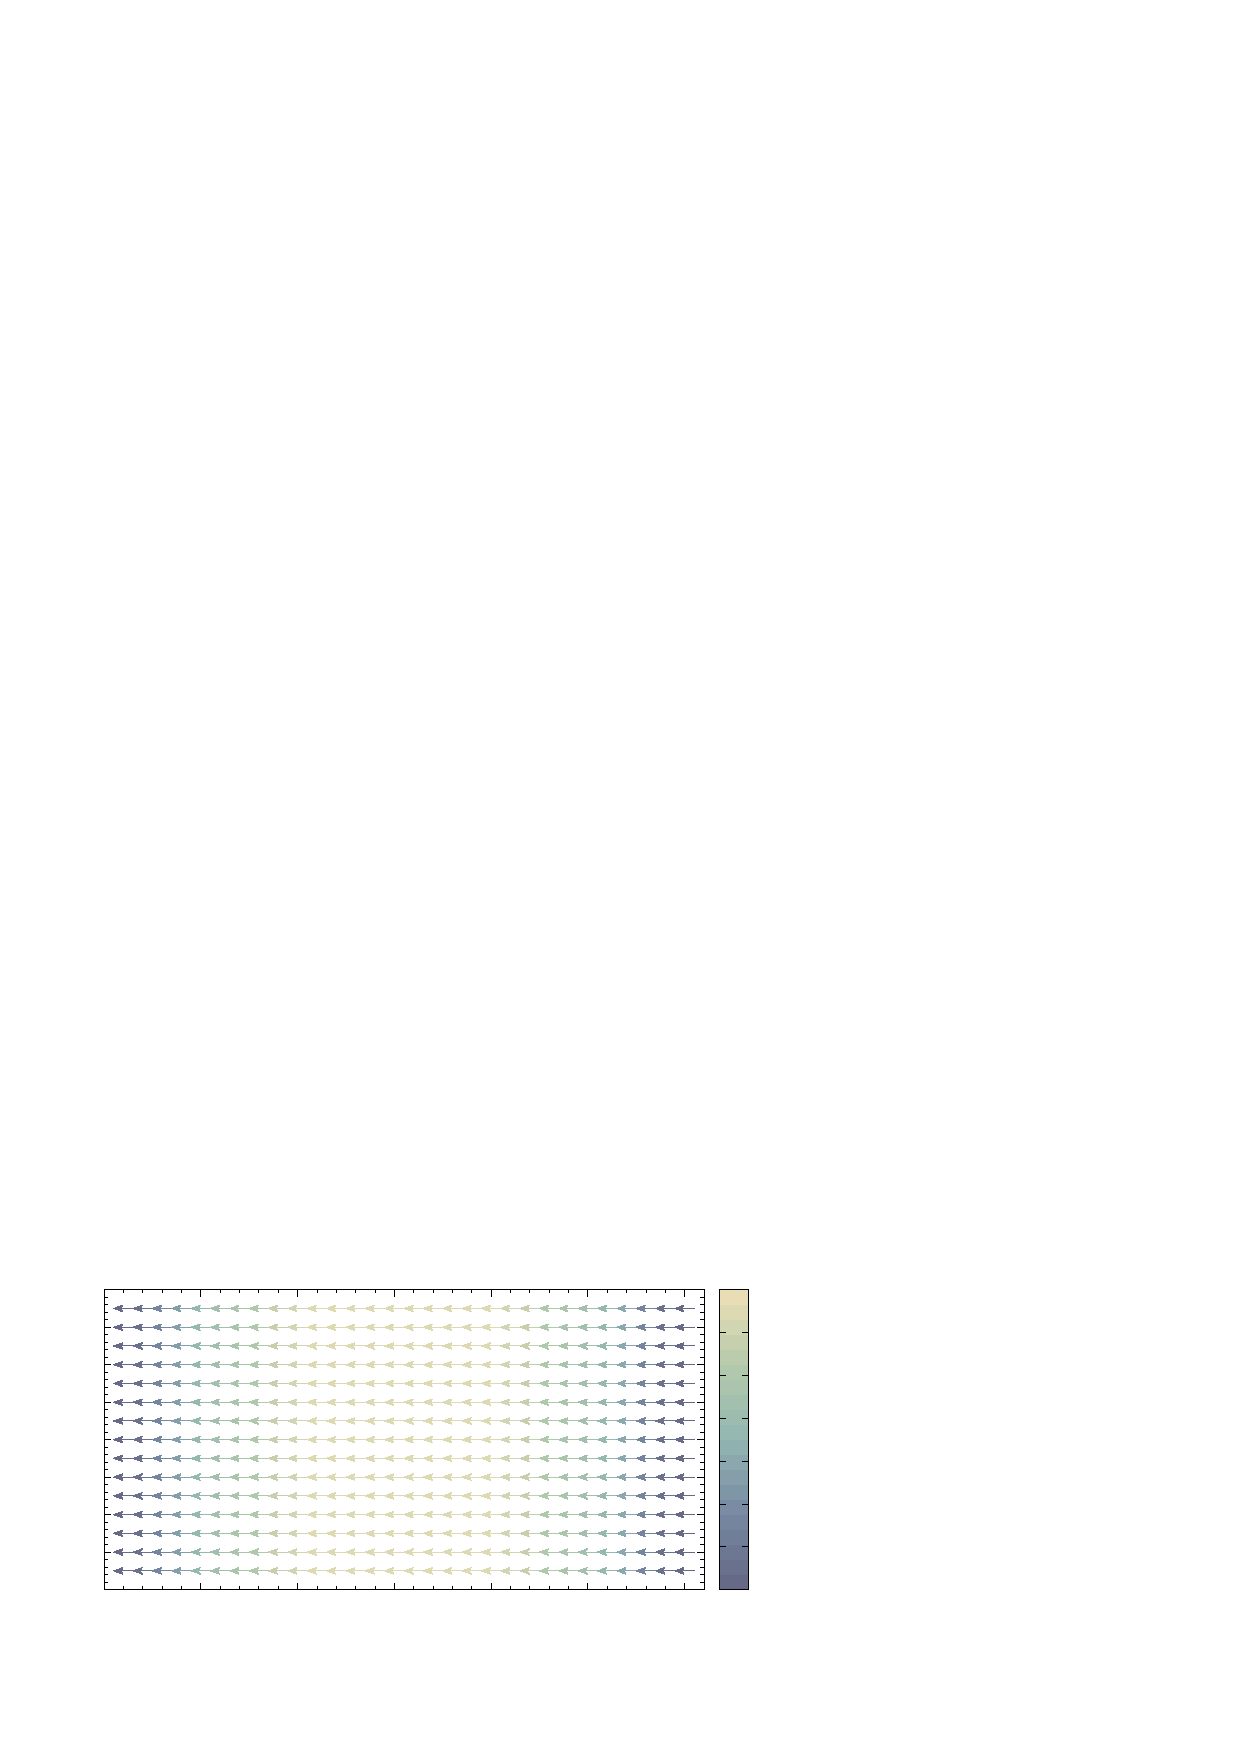
\includegraphics[width={288.00bp},height={188.60bp}]{Plots/SC10AM10/HeatMap/VertHorizBC/plot}}%
    \gplfronttext
  \end{picture}%
\endgroup


%         \caption{Surrounded with vaccuum.}
%         \label{fig:first}
%     \end{subfigure}\\
%     \begin{subfigure}{0.45\textwidth}
%         \centering
%         % GNUPLOT: LaTeX picture with Postscript
\begingroup
  % Encoding inside the plot.  In the header of your document, this encoding
  % should to defined, e.g., by using
  % \usepackage[cp1252,<other encodings>]{inputenc}
  \inputencoding{cp1252}%
  \makeatletter
  \providecommand\color[2][]{%
    \GenericError{(gnuplot) \space\space\space\@spaces}{%
      Package color not loaded in conjunction with
      terminal option `colourtext'%
    }{See the gnuplot documentation for explanation.%
    }{Either use 'blacktext' in gnuplot or load the package
      color.sty in LaTeX.}%
    \renewcommand\color[2][]{}%
  }%
  \providecommand\includegraphics[2][]{%
    \GenericError{(gnuplot) \space\space\space\@spaces}{%
      Package graphicx or graphics not loaded%
    }{See the gnuplot documentation for explanation.%
    }{The gnuplot epslatex terminal needs graphicx.sty or graphics.sty.}%
    \renewcommand\includegraphics[2][]{}%
  }%
  \providecommand\rotatebox[2]{#2}%
  \@ifundefined{ifGPcolor}{%
    \newif\ifGPcolor
    \GPcolortrue
  }{}%
  \@ifundefined{ifGPblacktext}{%
    \newif\ifGPblacktext
    \GPblacktextfalse
  }{}%
  % define a \g@addto@macro without @ in the name:
  \let\gplgaddtomacro\g@addto@macro
  % define empty templates for all commands taking text:
  \gdef\gplbacktext{}%
  \gdef\gplfronttext{}%
  \makeatother
  \ifGPblacktext
    % no textcolor at all
    \def\colorrgb#1{}%
    \def\colorgray#1{}%
  \else
    % gray or color?
    \ifGPcolor
      \def\colorrgb#1{\color[rgb]{#1}}%
      \def\colorgray#1{\color[gray]{#1}}%
      \expandafter\def\csname LTw\endcsname{\color{white}}%
      \expandafter\def\csname LTb\endcsname{\color{black}}%
      \expandafter\def\csname LTa\endcsname{\color{black}}%
      \expandafter\def\csname LT0\endcsname{\color[rgb]{1,0,0}}%
      \expandafter\def\csname LT1\endcsname{\color[rgb]{0,1,0}}%
      \expandafter\def\csname LT2\endcsname{\color[rgb]{0,0,1}}%
      \expandafter\def\csname LT3\endcsname{\color[rgb]{1,0,1}}%
      \expandafter\def\csname LT4\endcsname{\color[rgb]{0,1,1}}%
      \expandafter\def\csname LT5\endcsname{\color[rgb]{1,1,0}}%
      \expandafter\def\csname LT6\endcsname{\color[rgb]{0,0,0}}%
      \expandafter\def\csname LT7\endcsname{\color[rgb]{1,0.3,0}}%
      \expandafter\def\csname LT8\endcsname{\color[rgb]{0.5,0.5,0.5}}%
    \else
      % gray
      \def\colorrgb#1{\color{black}}%
      \def\colorgray#1{\color[gray]{#1}}%
      \expandafter\def\csname LTw\endcsname{\color{white}}%
      \expandafter\def\csname LTb\endcsname{\color{black}}%
      \expandafter\def\csname LTa\endcsname{\color{black}}%
      \expandafter\def\csname LT0\endcsname{\color{black}}%
      \expandafter\def\csname LT1\endcsname{\color{black}}%
      \expandafter\def\csname LT2\endcsname{\color{black}}%
      \expandafter\def\csname LT3\endcsname{\color{black}}%
      \expandafter\def\csname LT4\endcsname{\color{black}}%
      \expandafter\def\csname LT5\endcsname{\color{black}}%
      \expandafter\def\csname LT6\endcsname{\color{black}}%
      \expandafter\def\csname LT7\endcsname{\color{black}}%
      \expandafter\def\csname LT8\endcsname{\color{black}}%
    \fi
  \fi
    \setlength{\unitlength}{0.0500bp}%
    \ifx\gptboxheight\undefined%
      \newlength{\gptboxheight}%
      \newlength{\gptboxwidth}%
      \newsavebox{\gptboxtext}%
    \fi%
    \setlength{\fboxrule}{0.5pt}%
    \setlength{\fboxsep}{1pt}%
    \definecolor{tbcol}{rgb}{1,1,1}%
\begin{picture}(5760.00,3772.00)%
    \gplgaddtomacro\gplbacktext{%
      \csname LTb\endcsname%%
      \put(1807,3313){\makebox(0,0){\strut{}SC}}%
      \put(3953,3313){\makebox(0,0){\strut{}AM}}%
    }%
    \gplgaddtomacro\gplfronttext{%
      \csname LTb\endcsname%%
      \put(1073,742){\makebox(0,0){\scriptsize 2}}%
      \put(1525,742){\makebox(0,0){\scriptsize 4}}%
      \put(1977,742){\makebox(0,0){\scriptsize 6}}%
      \put(2429,742){\makebox(0,0){\scriptsize 8}}%
      \put(2880,742){\makebox(0,0){\scriptsize 10}}%
      \put(3331,742){\makebox(0,0){\scriptsize 12}}%
      \put(3783,742){\makebox(0,0){\scriptsize 14}}%
      \put(4235,742){\makebox(0,0){\scriptsize 16}}%
      \put(4687,742){\makebox(0,0){\scriptsize 18}}%
      \put(2880,478){\makebox(0,0){\small\textbf{Lattice site $i_x$ in $\bm{e}_x$}}}%
      \put(480,1006){\makebox(0,0){\scriptsize 2}}%
      \put(480,1254){\makebox(0,0){\scriptsize 4}}%
      \put(480,1501){\makebox(0,0){\scriptsize 6}}%
      \put(480,1749){\makebox(0,0){\scriptsize 8}}%
      \put(480,1996){\makebox(0,0){\scriptsize 10}}%
      \put(480,2243){\makebox(0,0){\scriptsize 12}}%
      \put(480,2491){\makebox(0,0){\scriptsize 14}}%
      \put(480,2738){\makebox(0,0){\scriptsize 16}}%
      \put(480,2986){\makebox(0,0){\scriptsize 18}}%
      \put(150,1996){\rotatebox{-270.00}{\makebox(0,0){\small\textbf{Lattice site $i_y$ in $\bm{e}_y$}}}}%
      \put(5743,820){\makebox(0,0){\tiny \(0\)}}%
      \put(5743,1212){\makebox(0,0){\tiny \(1e{-06}\)}}%
      \put(5743,1604){\makebox(0,0){\tiny \(2e{-06}\)}}%
      \put(5743,1996){\makebox(0,0){\tiny \(3e{-06}\)}}%
      \put(5743,2388){\makebox(0,0){\tiny \(4e{-06}\)}}%
      \put(5743,2780){\makebox(0,0){\tiny \(5e{-06}\)}}%
      \put(5743,3171){\makebox(0,0){\tiny \(6e{-06}\)}}%
    }%
    \gplbacktext
    \put(0,0){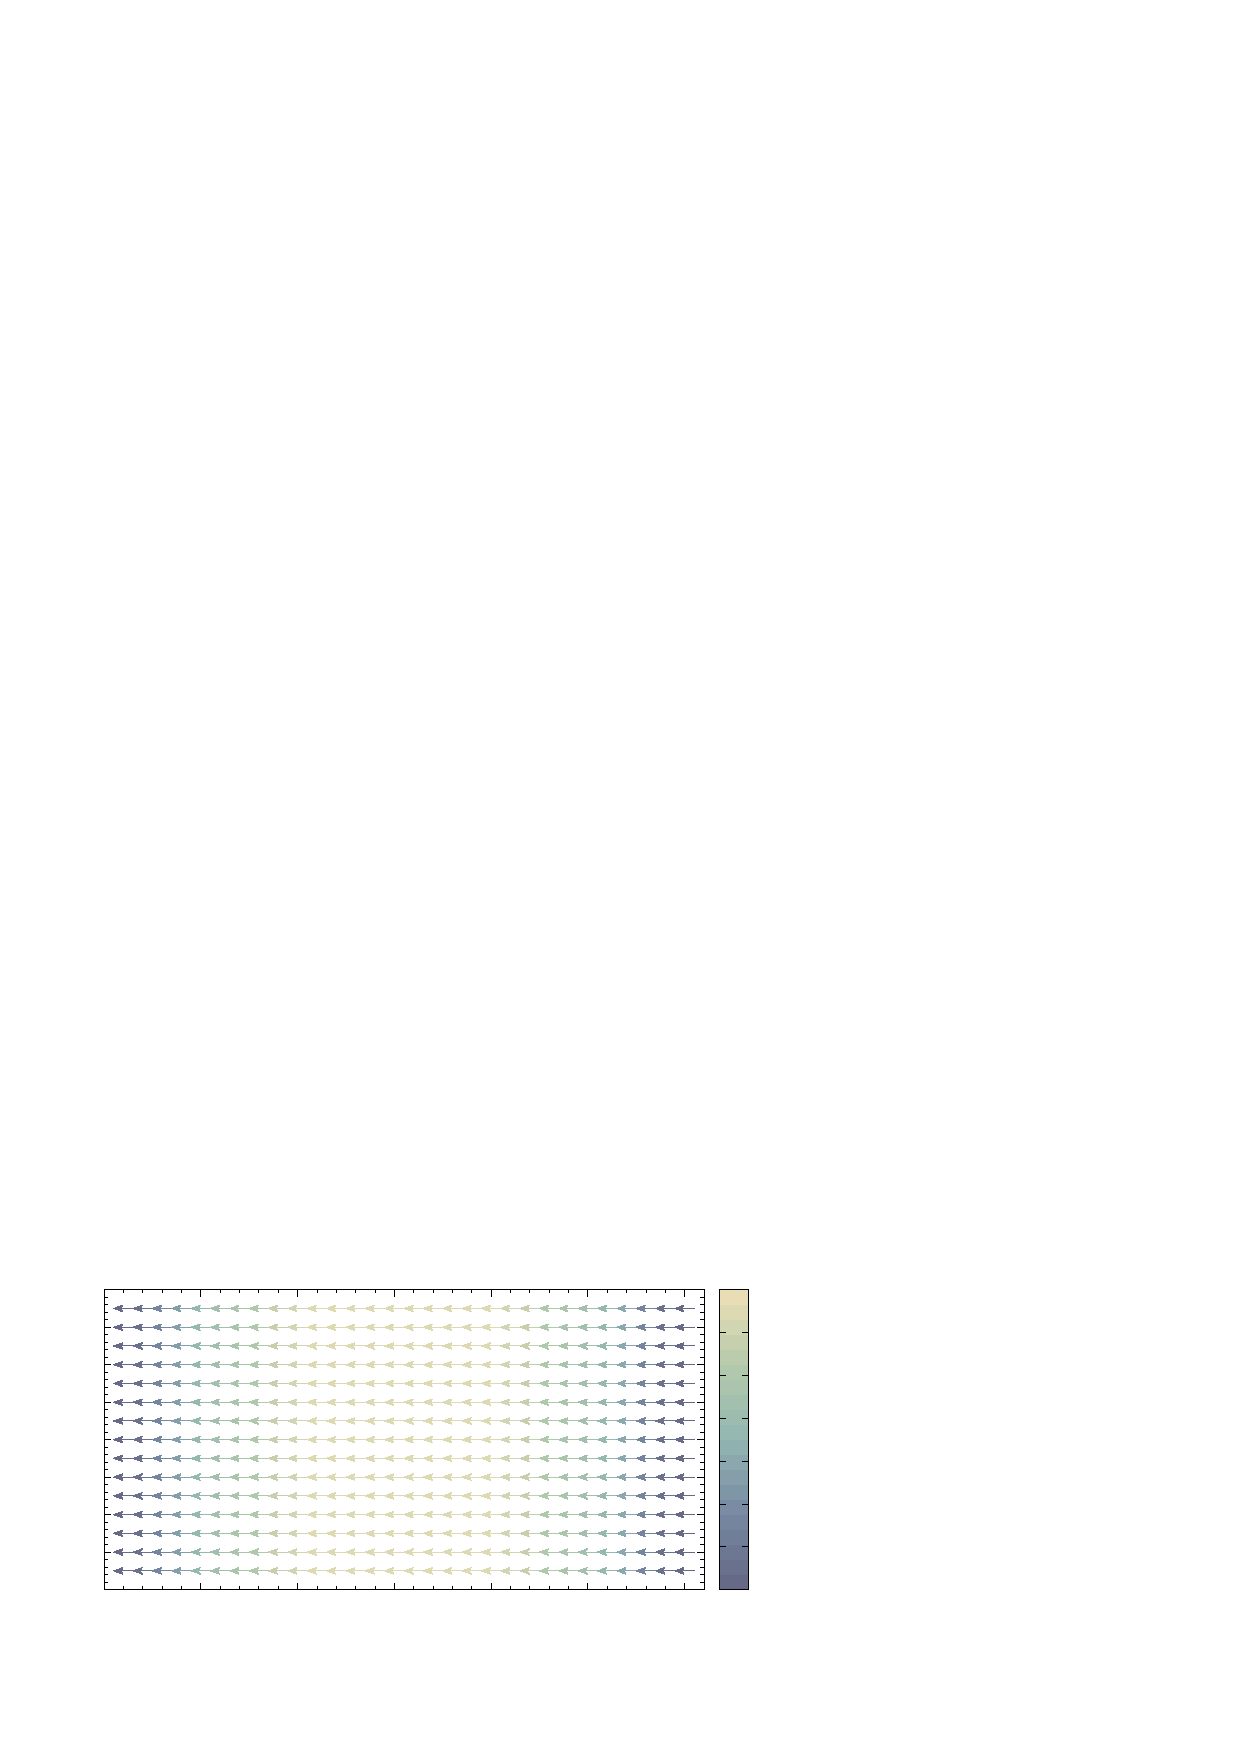
\includegraphics[width={288.00bp},height={188.60bp}]{Plots/SC10AM10/HeatMap/VertHorizBC/plot}}%
    \gplfronttext
  \end{picture}%
\endgroup


%         \caption{Vaccum on the right and left with vertical periodic boundary conditions.}
%         \label{fig:first}
%     \end{subfigure}
%     \begin{subfigure}{0.45\textwidth}
%         \centering
%         % GNUPLOT: LaTeX picture with Postscript
\begingroup
  % Encoding inside the plot.  In the header of your document, this encoding
  % should to defined, e.g., by using
  % \usepackage[cp1252,<other encodings>]{inputenc}
  \inputencoding{cp1252}%
  \makeatletter
  \providecommand\color[2][]{%
    \GenericError{(gnuplot) \space\space\space\@spaces}{%
      Package color not loaded in conjunction with
      terminal option `colourtext'%
    }{See the gnuplot documentation for explanation.%
    }{Either use 'blacktext' in gnuplot or load the package
      color.sty in LaTeX.}%
    \renewcommand\color[2][]{}%
  }%
  \providecommand\includegraphics[2][]{%
    \GenericError{(gnuplot) \space\space\space\@spaces}{%
      Package graphicx or graphics not loaded%
    }{See the gnuplot documentation for explanation.%
    }{The gnuplot epslatex terminal needs graphicx.sty or graphics.sty.}%
    \renewcommand\includegraphics[2][]{}%
  }%
  \providecommand\rotatebox[2]{#2}%
  \@ifundefined{ifGPcolor}{%
    \newif\ifGPcolor
    \GPcolortrue
  }{}%
  \@ifundefined{ifGPblacktext}{%
    \newif\ifGPblacktext
    \GPblacktextfalse
  }{}%
  % define a \g@addto@macro without @ in the name:
  \let\gplgaddtomacro\g@addto@macro
  % define empty templates for all commands taking text:
  \gdef\gplbacktext{}%
  \gdef\gplfronttext{}%
  \makeatother
  \ifGPblacktext
    % no textcolor at all
    \def\colorrgb#1{}%
    \def\colorgray#1{}%
  \else
    % gray or color?
    \ifGPcolor
      \def\colorrgb#1{\color[rgb]{#1}}%
      \def\colorgray#1{\color[gray]{#1}}%
      \expandafter\def\csname LTw\endcsname{\color{white}}%
      \expandafter\def\csname LTb\endcsname{\color{black}}%
      \expandafter\def\csname LTa\endcsname{\color{black}}%
      \expandafter\def\csname LT0\endcsname{\color[rgb]{1,0,0}}%
      \expandafter\def\csname LT1\endcsname{\color[rgb]{0,1,0}}%
      \expandafter\def\csname LT2\endcsname{\color[rgb]{0,0,1}}%
      \expandafter\def\csname LT3\endcsname{\color[rgb]{1,0,1}}%
      \expandafter\def\csname LT4\endcsname{\color[rgb]{0,1,1}}%
      \expandafter\def\csname LT5\endcsname{\color[rgb]{1,1,0}}%
      \expandafter\def\csname LT6\endcsname{\color[rgb]{0,0,0}}%
      \expandafter\def\csname LT7\endcsname{\color[rgb]{1,0.3,0}}%
      \expandafter\def\csname LT8\endcsname{\color[rgb]{0.5,0.5,0.5}}%
    \else
      % gray
      \def\colorrgb#1{\color{black}}%
      \def\colorgray#1{\color[gray]{#1}}%
      \expandafter\def\csname LTw\endcsname{\color{white}}%
      \expandafter\def\csname LTb\endcsname{\color{black}}%
      \expandafter\def\csname LTa\endcsname{\color{black}}%
      \expandafter\def\csname LT0\endcsname{\color{black}}%
      \expandafter\def\csname LT1\endcsname{\color{black}}%
      \expandafter\def\csname LT2\endcsname{\color{black}}%
      \expandafter\def\csname LT3\endcsname{\color{black}}%
      \expandafter\def\csname LT4\endcsname{\color{black}}%
      \expandafter\def\csname LT5\endcsname{\color{black}}%
      \expandafter\def\csname LT6\endcsname{\color{black}}%
      \expandafter\def\csname LT7\endcsname{\color{black}}%
      \expandafter\def\csname LT8\endcsname{\color{black}}%
    \fi
  \fi
    \setlength{\unitlength}{0.0500bp}%
    \ifx\gptboxheight\undefined%
      \newlength{\gptboxheight}%
      \newlength{\gptboxwidth}%
      \newsavebox{\gptboxtext}%
    \fi%
    \setlength{\fboxrule}{0.5pt}%
    \setlength{\fboxsep}{1pt}%
    \definecolor{tbcol}{rgb}{1,1,1}%
\begin{picture}(5760.00,3772.00)%
    \gplgaddtomacro\gplbacktext{%
      \csname LTb\endcsname%%
      \put(1807,3313){\makebox(0,0){\strut{}SC}}%
      \put(3953,3313){\makebox(0,0){\strut{}AM}}%
    }%
    \gplgaddtomacro\gplfronttext{%
      \csname LTb\endcsname%%
      \put(1073,742){\makebox(0,0){\scriptsize 2}}%
      \put(1525,742){\makebox(0,0){\scriptsize 4}}%
      \put(1977,742){\makebox(0,0){\scriptsize 6}}%
      \put(2429,742){\makebox(0,0){\scriptsize 8}}%
      \put(2880,742){\makebox(0,0){\scriptsize 10}}%
      \put(3331,742){\makebox(0,0){\scriptsize 12}}%
      \put(3783,742){\makebox(0,0){\scriptsize 14}}%
      \put(4235,742){\makebox(0,0){\scriptsize 16}}%
      \put(4687,742){\makebox(0,0){\scriptsize 18}}%
      \put(2880,478){\makebox(0,0){\small\textbf{Lattice site $i_x$ in $\bm{e}_x$}}}%
      \put(480,1006){\makebox(0,0){\scriptsize 2}}%
      \put(480,1254){\makebox(0,0){\scriptsize 4}}%
      \put(480,1501){\makebox(0,0){\scriptsize 6}}%
      \put(480,1749){\makebox(0,0){\scriptsize 8}}%
      \put(480,1996){\makebox(0,0){\scriptsize 10}}%
      \put(480,2243){\makebox(0,0){\scriptsize 12}}%
      \put(480,2491){\makebox(0,0){\scriptsize 14}}%
      \put(480,2738){\makebox(0,0){\scriptsize 16}}%
      \put(480,2986){\makebox(0,0){\scriptsize 18}}%
      \put(150,1996){\rotatebox{-270.00}{\makebox(0,0){\small\textbf{Lattice site $i_y$ in $\bm{e}_y$}}}}%
      \put(5743,820){\makebox(0,0){\tiny \(0\)}}%
      \put(5743,1212){\makebox(0,0){\tiny \(1e{-06}\)}}%
      \put(5743,1604){\makebox(0,0){\tiny \(2e{-06}\)}}%
      \put(5743,1996){\makebox(0,0){\tiny \(3e{-06}\)}}%
      \put(5743,2388){\makebox(0,0){\tiny \(4e{-06}\)}}%
      \put(5743,2780){\makebox(0,0){\tiny \(5e{-06}\)}}%
      \put(5743,3171){\makebox(0,0){\tiny \(6e{-06}\)}}%
    }%
    \gplbacktext
    \put(0,0){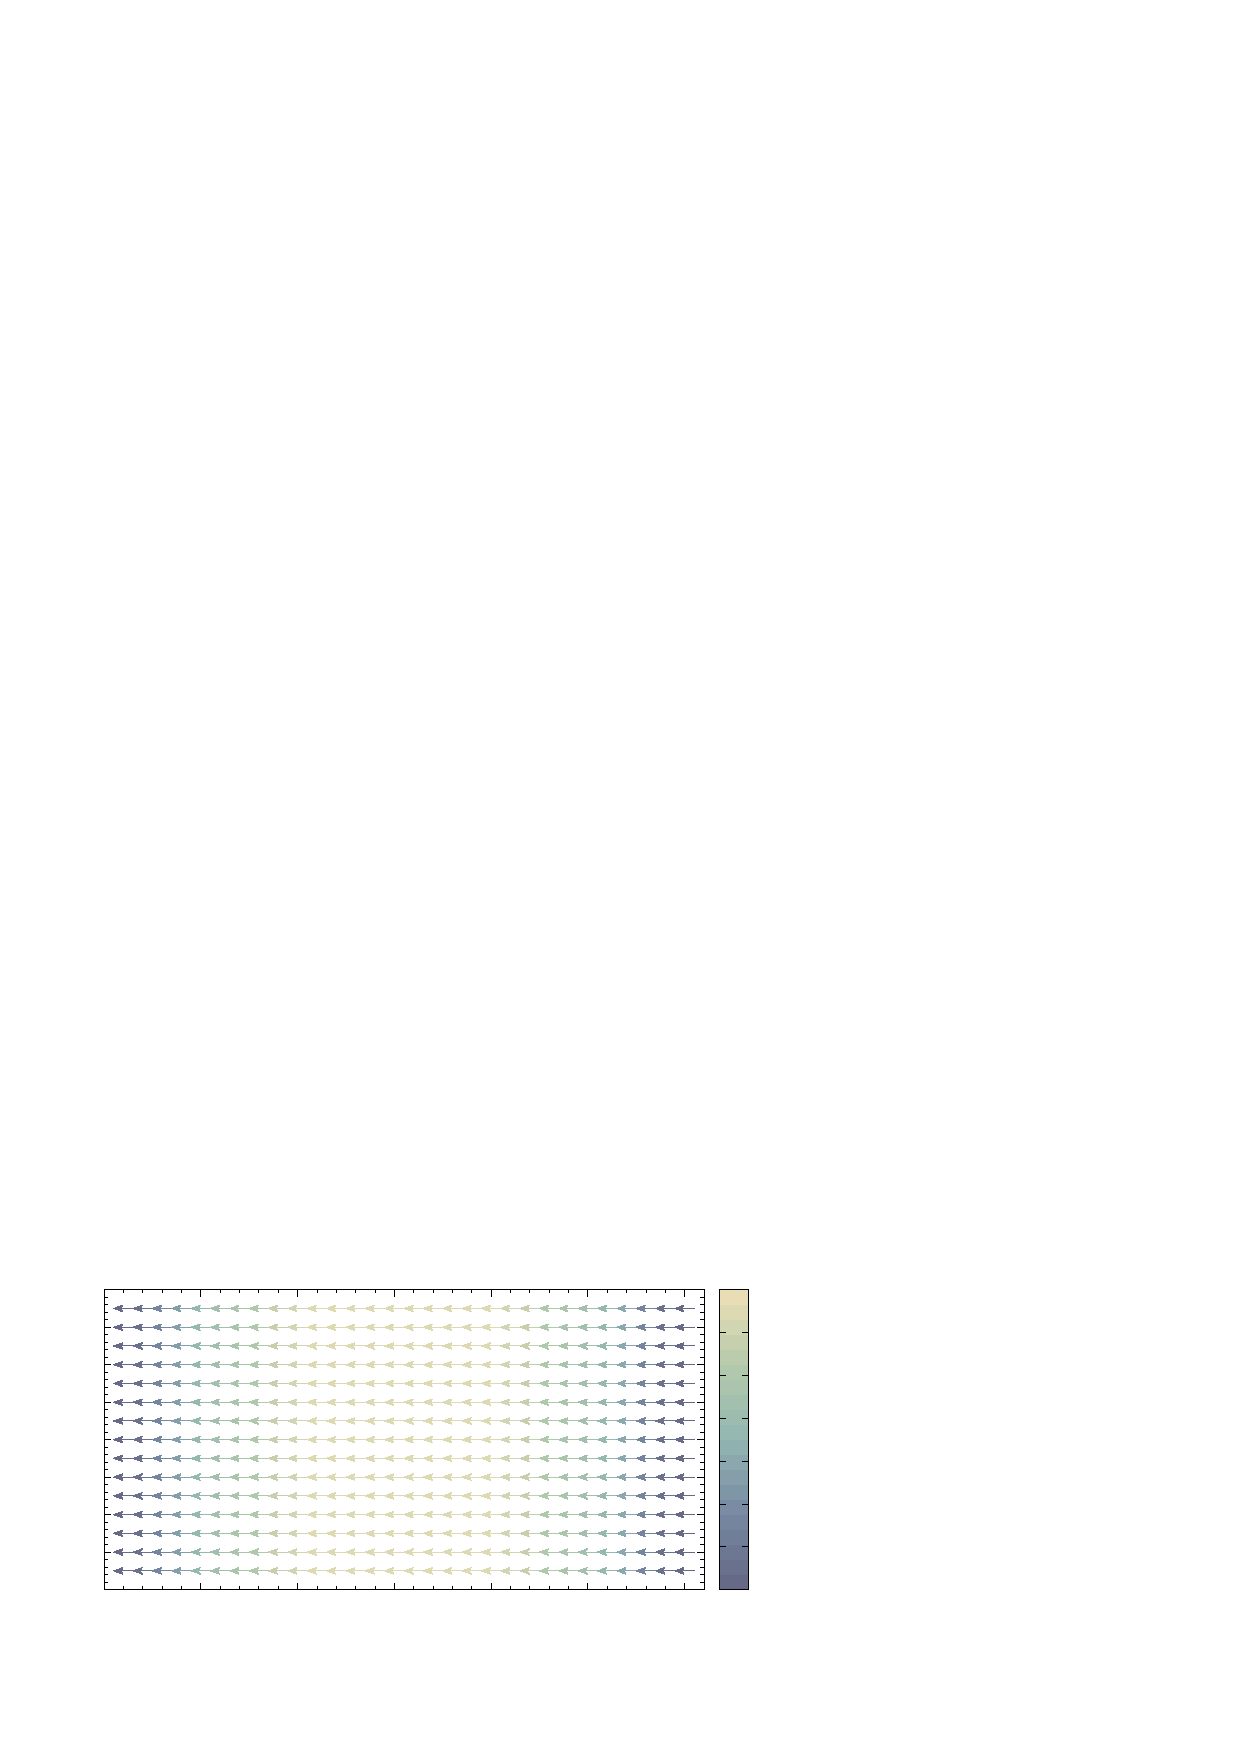
\includegraphics[width={288.00bp},height={188.60bp}]{Plots/SC10AM10/HeatMap/VertHorizBC/plot}}%
    \gplfronttext
  \end{picture}%
\endgroup


%         \caption{Both vertical and horizontal periodic boundary conditions.}
%         \label{fig:first}
%     \end{subfigure}
%     \caption{Heatmaps of the correlation function $|\langle c_{i\uparrow} c_{i\downarrow}\rangle|$ for different boundary conditions.}
% \end{figure}
\end{document}